% Misión 4: la geocerca del concierto. Portada y vuelo paso a paso.
% La caja en NED: norte -6..14, este -10..10, hasta 8 m. El escenario queda al norte.
% vuelo_prueba sale al norte a 5.5 m/s; el guardián lo para con Hold y lo regresa con Return.

\begin{frame}{Misión 4: la geocerca del concierto}
  \begin{columns}[c]
    \column{0.56\textwidth}
    \begin{tikzpicture}
      \node[inner sep=0] (im) {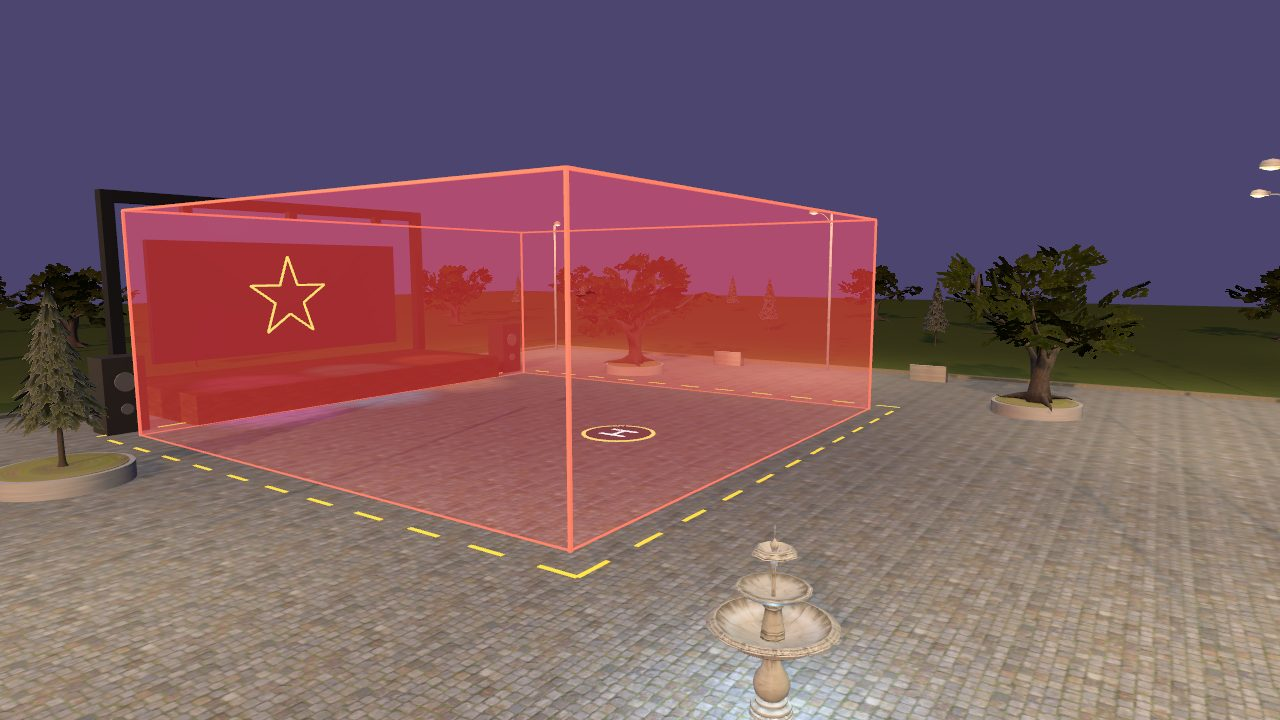
\includegraphics[width=\linewidth]{plaza_concierto}};
      \node[anchor=north west,fill=azul,text=white,font=\bfseries\scriptsize,rounded corners=2pt]
        at ([xshift=4pt,yshift=-4pt]im.north west) {MISIÓN 4 · NIVEL 2 \nivel{2}};
    \end{tikzpicture}\\[0.3em]
    \small\textbf{Escenario}: sobre un concierto el dron no puede salir de una caja de
    20\,$\times$\,20\,$\times$\,8 m. Un \textbf{guardián} que no vuela lo vigila, lo vuele quien lo vuele.
    \column{0.41\textwidth}
    \ficha{x500_volando}{x500}{plaza\_concierto}{guardian\_geocerca}{\cmd{flight\_mode\_monitor} y
      \cmd{return\_home}}{\textbf{predecir} dónde se va a detener}{no rebasa la cerca más de 1 m}
  \end{columns}
\end{frame}

\begin{frame}{El guardián, paso a paso}
  \begin{columns}[c]
    \column{0.47\textwidth}\centering
    \begin{tikzpicture}[scale=0.21]
      \fill[gray!35] (-8,14) rectangle (8,21); \node[font=\tiny] at (0,17.5) {escenario};
      \draw[orange,dashed,thick] (-11,-7) rectangle (11,15);
      \draw[rojo,thick,fill=red!6] (-10,-6) rectangle (10,14);
      \node[draw,circle,fill=azulclaro,inner sep=0.3pt,font=\tiny] at (0,0) {H};
      \draw[-{Stealth},verde,thick] (-9,-4) -- (-9,0) node[above,font=\tiny] {N};
      % dónde está el dron, su flecha de velocidad y dónde se detendría
      \only<1>{\node at (0,0) {\dronarriba{0.75cm}};}
      \only<2>{\node at (0,3) {\dronarriba{0.75cm}}; \draw[-{Stealth},azul,thick] (0,4.3) -- (0,6.3);
        \fill[gris] (0,9) circle (10pt); \draw[gris,dashed] (0,4.3) -- (0,9);}
      \only<3>{\node at (0,8.9) {\dronarriba{0.75cm}}; \draw[-{Stealth},azul,thick] (0,10.2) -- (0,12.6);
        \fill[rojo] (0,19.2) circle (12pt); \draw[rojo,dashed,thick] (0,10.2) -- (0,19.2);}
      \only<4>{\node at (0,13.4) {\dronarriba{0.75cm}};}
      \only<5>{\node at (0,13.4) {\dronarriba{0.75cm}}; \draw[naranja,dashed,thick,-{Stealth}] (1.2,12.4) -- (1.2,1.2);}
      \only<6>{\node at (0,0) {\dronarriba{0.75cm}};}
      \node[font=\tiny,text=gris,visible on=<2>] at (4.2,9) {se detendría aquí};
      \node[font=\tiny,text=rojo,visible on=<3>] at (4.6,19.2) {¡afuera!};
    \end{tikzpicture}
    \column{0.52\textwidth}
    \estados{1-2/WATCH,3-4/BRAKING,5/RETURNING,6/DONE}
    \vspace{0.3em}

    \only<1>{\begin{terminal}{guardian\_geocerca}
Guardián listo: norte -6..14, este -10..10, hasta 8 m
    \end{terminal}\small En otra terminal, \cmd{vuelo\_prueba} despega: es el ``piloto travieso'' que se va
      a lanzar al norte sin frenar.}%
    \only<2>{\begin{terminal}{guardian\_geocerca}
vigilando: a 11.0 m de la orilla, 4.0 m/s
    \end{terminal}\small Cada ciclo predice \textbf{dónde se detendría} si frenara ya ({\color{gris}$\bullet$}):
      $v\,t_r + v^2/2a$. Todavía cae adentro.}%
    \only<3>{\begin{terminal}{guardian\_geocerca}
¡Se va a salir! (a 5.1 m de la orilla,\\
\ va a 5.5 m/s): Hold
    \end{terminal}\small Está a 5 m de la orilla, pero \textbf{a 5.5 m/s se detendría afuera}
      ({\color{rojo}$\bullet$}). \textbf{Tu TODO}: pedir Hold \emph{ahora}, no cuando ya cruzó.}%
    \only<4>{\small\textbf{Frenando} (Hold). Se detiene justo antes de la cerca. Si esperaras a que cruzara la
      línea, se pasaría \textasciitilde10 m.}%
    \only<5>{\begin{terminal}{guardian\_geocerca}
Detenido a 0.00 m fuera. Return
    \end{terminal}\small Ya casi quieto y en Hold: \textbf{Return} (tu otro TODO).}%
    \only<6>{\begin{terminal}{guardian\_geocerca}
Aterrizó. Lo más que se salió de la cerca:\\
\ \ 0.00 m (límite 1.0) OK\\
Misión cumplida
    \end{terminal}}%
  \end{columns}
\end{frame}
